% vim: set tw=78 sts=2 sw=2 ts=8 aw et ai:

\begin{figure}[t]
\centering
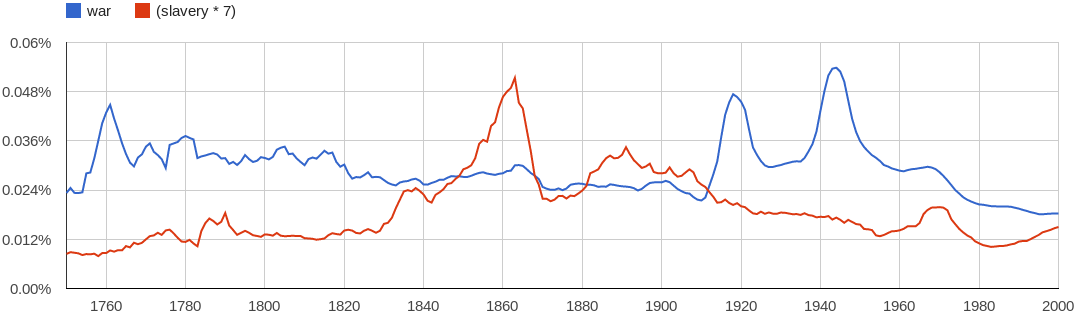
\includegraphics[max size={0.5 \textwidth}{0.5 \textheight}]{war-series}
\caption{Ngram time series for war and slavery}
\label{fig:war-series}
\end{figure}

%\begin{figure*}[ht]
%\centering
%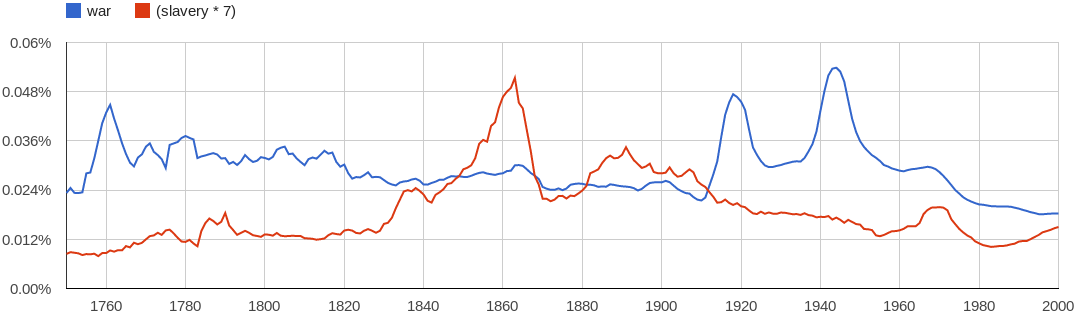
\includegraphics[max size={0.7 \textwidth}{0.7 \textheight}]{war-series}
%\caption{Ngram time series for war and slavery}
%\label{fig:war-series}
%\end{figure*}

Looking at the time series of n-gram \textit{war} shown in Figure~\ref{fig:war-series}, one can observe several well-defined peaks, corresponding to historic events like: Seven Years' War ($1755 - 1765$), World War I ($1910 - 1926$) and World War II ($1936 - 1953$). Further historic peaks, albeit less obvious, include War of Independence ($1775 - 1783$), American Civil War ($1860 - 1871$) and Vietnam War ($1961 - 1978$). A single plot can only reveal so much information, but by determining historical relevance for different n-grams and correlating the results, one can viably get a solid picture of a historic event.

The remainder of this section focuses on algorithms for peak detection that also measure the historical relevance. In future work, they shall be compared with similar methods of finding bursty features \newcite{He:2007:AFT:1277741.1277779}.

\subsubsection{Double Change Peak Detection}

Instead of performing full peak detection, it is simpler to find the portions of abrupt increase and decrease that form a peak. Formally, we say that a time series $\left\{ s_{i, t} \right\}$ suffers a double increase or decrease if it increases or decrease twice consecutively. Furthermore, the magnitude of that increase (Equation~\ref{eq:double-increase}) or decrease (Equation~\ref{eq:double-decrease}) at time $t$ is defined as the maximum $x \in \left[ 0, 1 \right]$ that satisfies one of the following equations:
\begin{align}
\label{eq:double-increase}
s_{i, t} > \left( 1 + x \right) s_{i, t - 1}, \, s_{i, t + 1} > \left( 1 + x \right) s_{i, t}
\\
\label{eq:double-decrease}
s_{i, t} < \left( 1 - x \right) s_{i, t - 1}, \, s_{i, t + 1} < \left( 1 - x \right) s_{i, t}
\end{align}

Furthermore, the magnitude of a single increase or of a single decrease at time $t$ is defined as the maximum $x \in \left[ 0, 1 \right]$ that satisfies one of: $s_{i, t} > \left( 1 + 2x \right) s_{i, t - 1}$ or $s_{i, t} < \left( 1 - 2x \right) s_{i, t - 1}$.

The magnitude $m_{i, t}$ of the change around a point $t$ is the maximum between the magnitude of the double change and that of the single change at that point. Finally, the historical relevance is $r_{i, t} = \min \left( \left\lfloor 10 m_{i, t} \right\rfloor, 9 \right)$.

\subsubsection{Linear Model Peak Detection}

One can also use a linear model for approximating portions of the time series. More precisely, one fits lines to the graph of the time series using linear regression, by considering larger and larger intervals until the error rises above a given threshold.

Thus, upon finding a maximal interval fitted by a line within a small error, the magnitude of the change on that interval is defined as a linear function of the logarithm of the slope. This choice is motivated by the wide range of values that the slope can take, forming a sort of heavy-tailed distribution. The historical relevance on that interval is computed as follows: $r_{i, t} = \max \left( \left\lfloor m_{i, t} \right\rfloor, 0 \right)$.

\subsubsection{Gaussian Model Peak Detection}

As peaks are usually shaped like a Gaussian distribution, let us consider a time interval $\left[ l, r \right] \subseteq \left[ 1500, 2008 \right]$ and its associated time series $\left\{ s_{i, t} \right\}_{t=l}^{r}$. Initially, one must normalize the series to get a probability distribution:

\begin{align}
\label{eq:gaussian-normalization}
g_{i, t} &= \frac{s_{i, t} - \min_{p \in \overline{l, r}} s_{i, p}}{\sum_{q = l}^{r} \left( s_{i, q} - \min_{p \in \overline{l, r}} s_{i, p} \right)}.
\end{align}

This is approximated by a normal distribution $N \left( \mu, \sigma \right)$ with the following parameters: $\mu = \sum_{t=l}^{r} g_{i, t} t$, $\sigma^2 = \sum_{t=l}^{r} g_{i, t} \left( t - \mu \right)^2$.

The similarity between $g_{i, t}$ and $N \left( \mu, \sigma \right)$ is computed using the earth mover's distance introduced in \newcite{rubner98metric}. Unfortunately, we have to consider all possible intervals $\left[ l, r \right] \subseteq \left[ 1500, 2008 \right]$, which leads to cubic complexity. As evidenced in \newcite{balanda88kurtosis}, kurtosis, which is defined in terms of the fourth moment about the mean $\mu_4$ as $\gamma_2 = \frac{\mu_4}{\sigma^4} - 3$, can be used to decide if a probability distribution looks like a Gaussian bell. Using trivial preprocessing of partial sums, we are able to efficiently determine intervals on which the kurtosis is close to $0$.

Next, we sort the remaining intervals in increasing order of the earth mover's distance to the Gaussian and process them. Intervals that intersect previously processed ones are simply ignored, which ensures that the intervals are disjoint.

Finally, we compute the magnitude of the change on an interval $\left[ l, r \right]$ as the percentage with which the Gaussian peak increases from its smallest value to its largest value:

\begin{align}
\label{eq:gaussian-magnitude}
m_i \left( \left[ l, r \right] \right) &= \frac{N \left( \mu, \sigma \right) \left( \mu \right) \cdot \sum_{q} \left( s_{i, q} - \min_{p} s_{i, p} \right)}{\min_{p} s_{i, p}}.
\end{align}

One way to define historical relevance is to assign it a constant value on the interval: $r_{i, t} = \left\lfloor 10 \cdot \min \left( m_i \left( \left[ l, r \right] \right), 1) \right) \right\rfloor$. Alternatively, one can assign variable relevance, using a widening parameter $\omega \in \left[ 1, \infty \right)$ as follows:

\begin{align}
\label{eq:gaussian-model-variable-relevance}
r_{i, t} \left( \omega \right) &= r_{i, t} \cdot \frac{N \left( \mu, \omega \sigma \right) \left( t \right)}{N \left( \mu, \omega \sigma \right) \left( \mu \right)}, \, \forall t \in \left[ l, r \right].
\end{align}

\subsubsection{Graphical Analysis}

\begin{figure}[t]
\centering
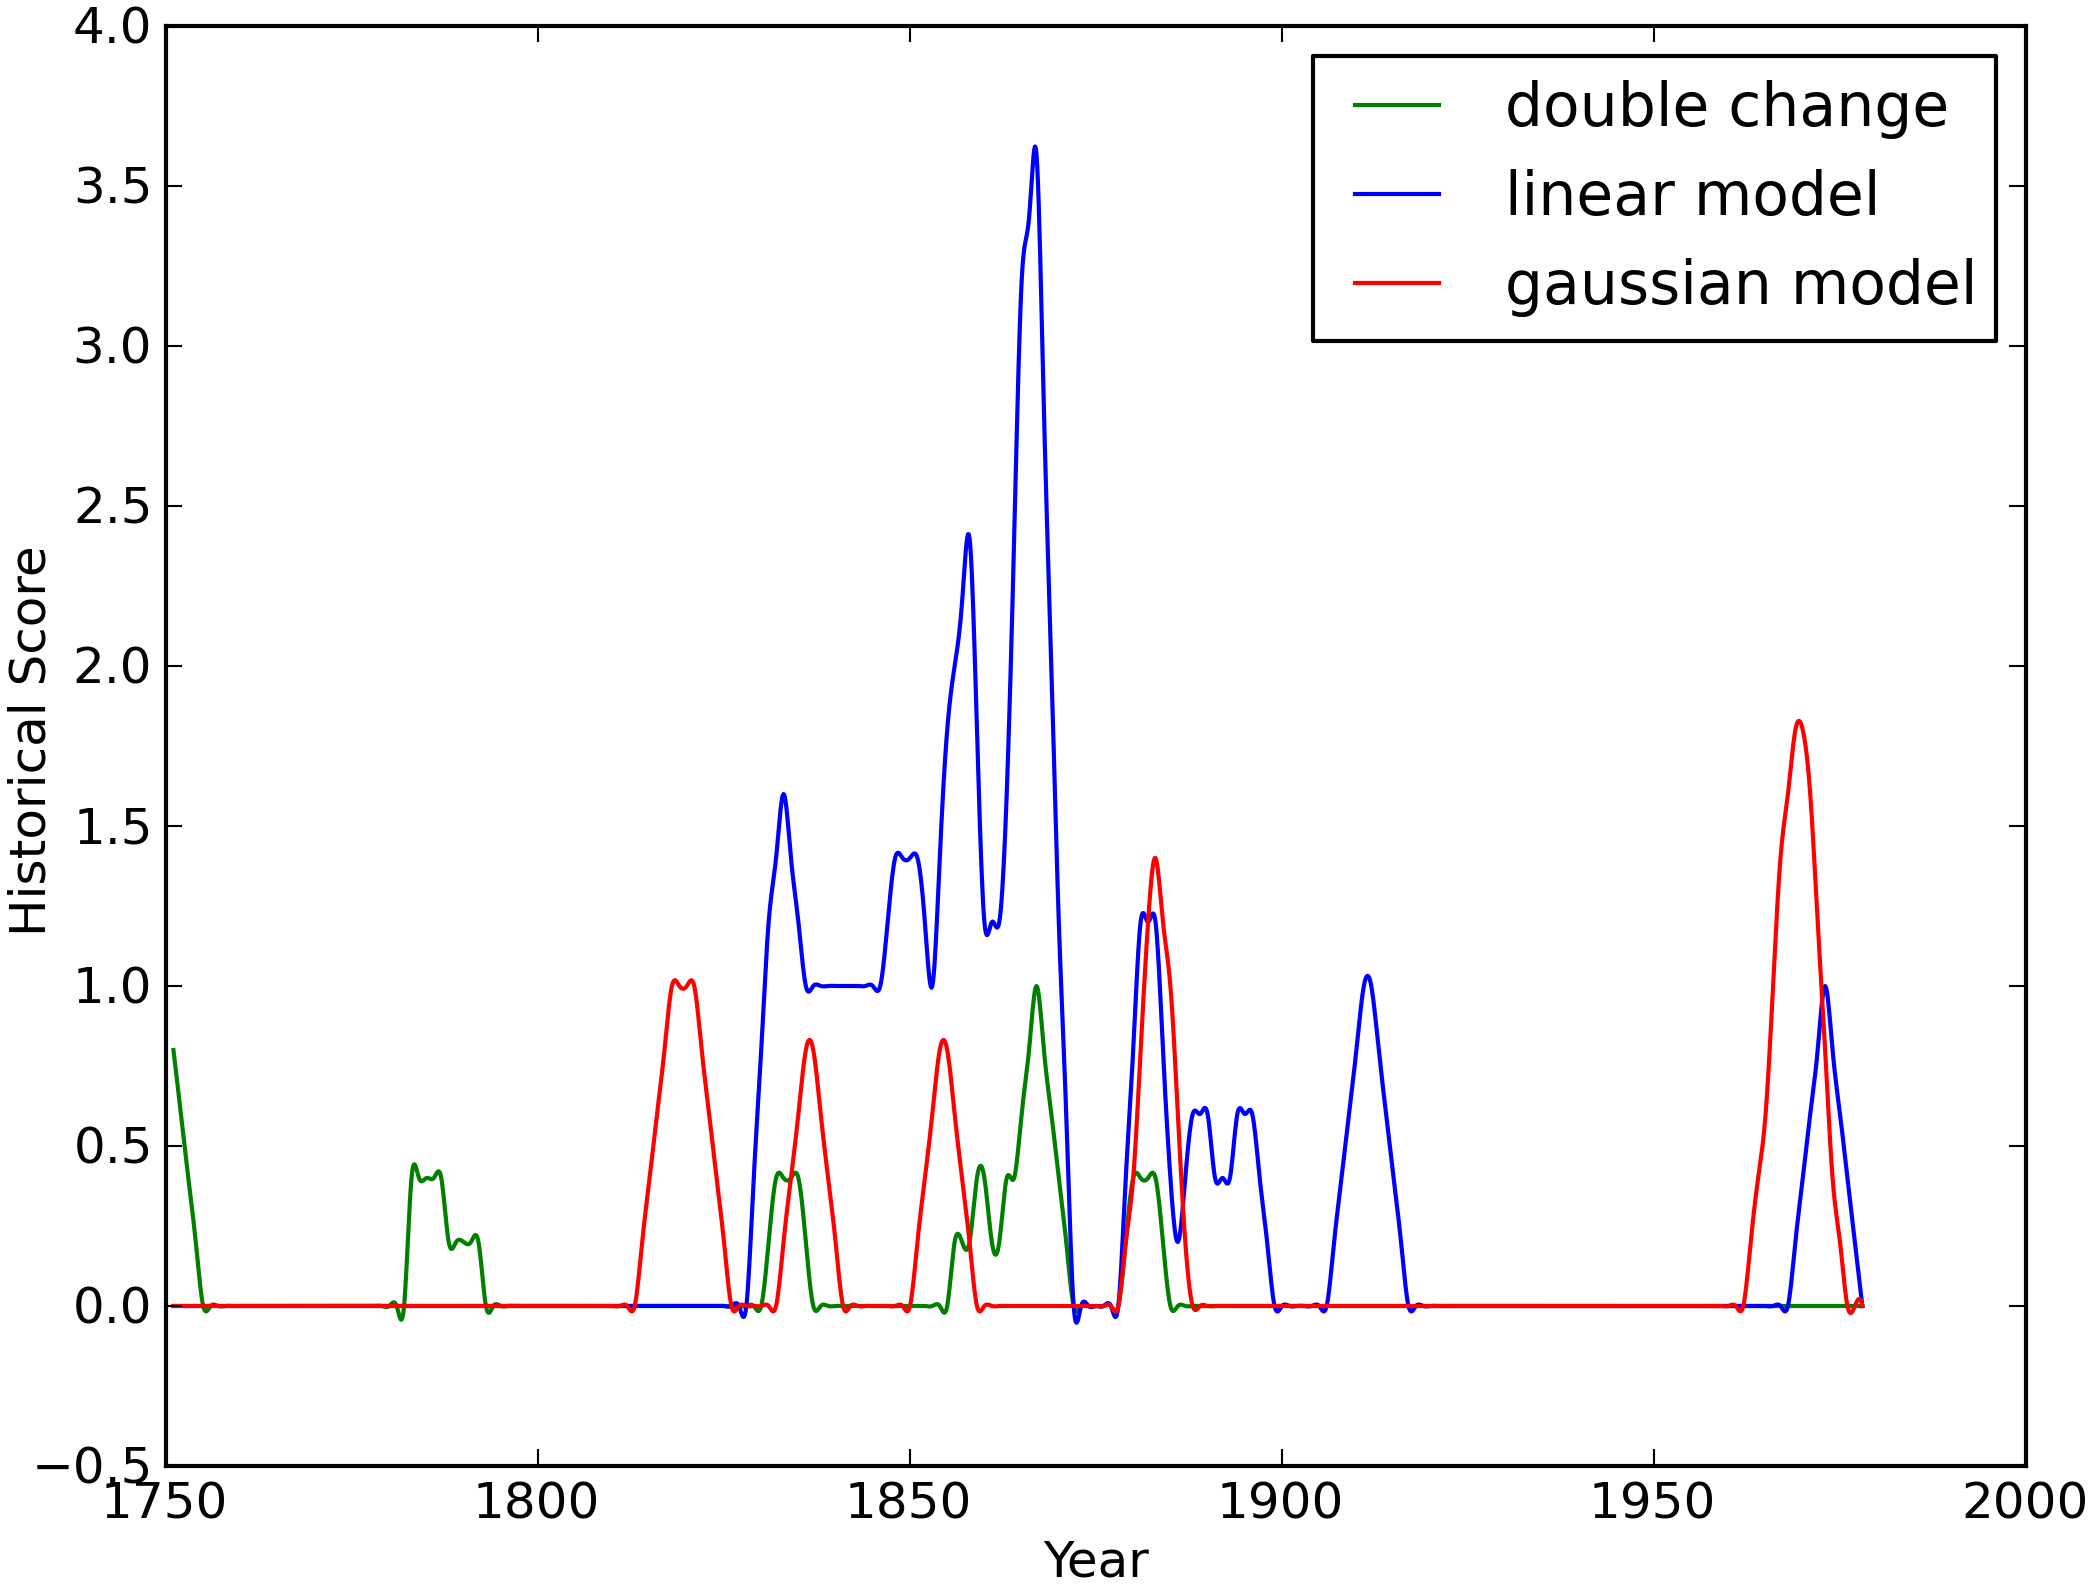
\includegraphics[max size={0.5 \textwidth}{0.5 \textheight}]{slavery-relevance}
\caption{Historical relevance of slavery}
\label{fig:slavery-relevance}
\end{figure}

The strengths and weaknesses of each of the algorithms can be analyzed using Figure~\ref{fig:slavery-relevance} (the Gaussian model uses $\omega = 2$). As can be seen in Figure~\ref{fig:war-series}, slavery has had two historic peaks: $1842 - 1871$ (the American Civil War) and $1964 - 1979$ (the African-American Civil Rights Movement).

The first peak is detected by all algorithms, but the best performer is the linear model, as the peak is triangular in shape. However, the Gaussian model does a better job at identifying the high point that probably corresponds to a historic event. The second peak is detected only by the last two algorithms. Since the peak is roughly bell-shaped, the Gaussian model performs better.

Lastly, the double change model also detects a minor peak centered around $1790$, when slavery became a hot issue as the Constitution of the United States was drafted. Thus, the double change model has the capability of detecting less important historic events.
